\section{Introduction}
In many machine learning applications, deep neural networks (DNNs) are utilized. In practice, when trying to improve the model's accuracy for the task at hand, multiple problems commonly arise: the amount of available data for training is often small relative to the amount of training data required under ideal circumstances, which usually causes over-fitting of the DNN. Additionally, training times when using DNNs can be long in general, limiting the feasibility of applying these methods in practice.
While, for most applications, it is often possible to push the measured accuracy to an acceptable level, some fields can benefit greatly from even higher prediction accuracy and robustness. To address this requirement, this work will introduce ensemble learning methods that can help tackle the before mentioned problems and improve the prediction performance. An ensemble combines multiple learners of the same or different types, producing a single learner with better performance than the single learners. These methods work exceptionally well when combining multiple learners with distinct weaknesses, as they can be combined to complement each other. \citep{Opitz.1999}


\section{Methods}

\subsection{Committee-based ensembles} \label{Committee}
In committee-based ensembles, the predictions of multiple individual learners are combined into a single prediction. This method can be applied to both classification and regression tasks.

% ----------------------------- VOTING -----------------------------
\subsubsection{Voting}

\begin{figure}[htbp]
    \centering
    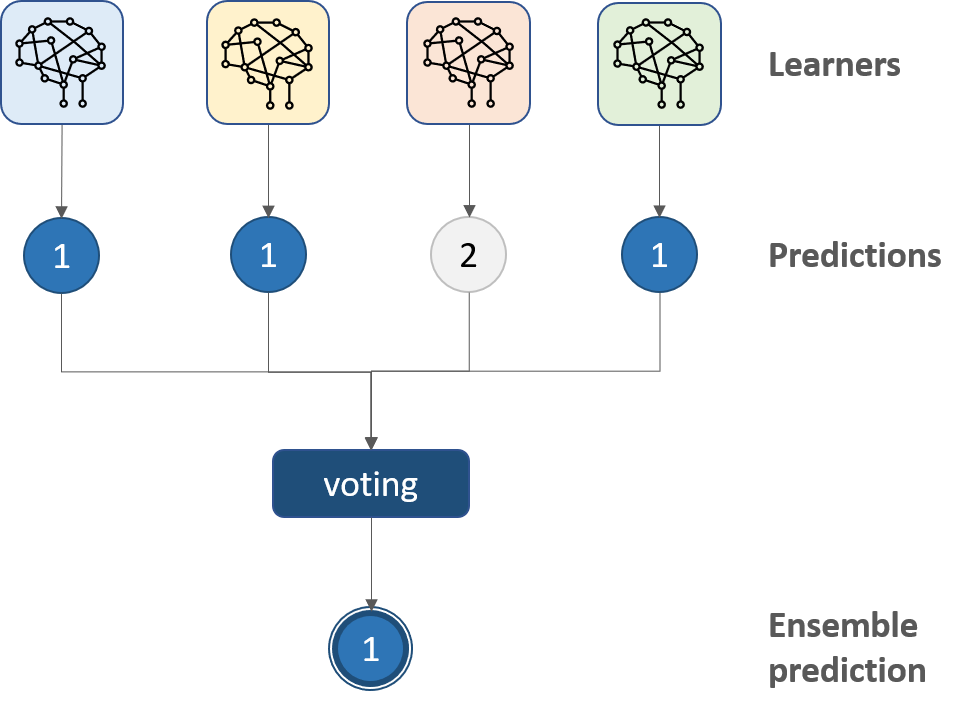
\includegraphics[width=.7\textwidth]{figures/voting}
    \caption{Symbolic representation of a voting ensemble.}
    \label{fig:voting}
\end{figure}

For classification tasks, voting ensembles are the most common. These combine the predictions of the individual learners by performing a majority vote. Often, the votes are weighted to prioritize learners that are known to make good decisions. Additionally, soft voting can be applied, where highly confident individual votes are assigned additional weight.

For binary classification, a weighted vote can be expressed as

\begin{align}
    G(x) = \mathrm{sign}\!\left(\sum^{M}_{m=1}\alpha_m G_m(x)\right)
    \label{eq:voting}
\end{align}

\noindent with the resulting prediction $G(x)$ being determined from the predictions of the $M$ individual learners $G_m(x)$, which are weighted via the factors $\alpha_m$. For each prediction, the sign represents the assigned class, and the absolute value represents the confidence.

\subsubsection{Averaging}
For regression tasks, voting ensembles are not easily applicable due to the continuous prediction space. Instead, averaging ensembles are used most often. These combine the predictions from the individual learners by averaging them. Like with voting ensembles, different weights are often assigned to the individual learners to weigh their influence on the final prediction based on their performance. The averaging ensemble can be expressed as

\begin{align}
    G(x) = \frac{1}{M} \sum^{M}_{m=1}\alpha_m G_m(x)
    \label{eq:averaging}
\end{align}

% ----------------------------- BAGGING -----------------------------
\subsection{Bagging} \label{Bagging}

\begin{figure}[htbp]
    \centering
    \includesvg[width=.7\textwidth]{figures/Ensemble_Bagging}
    \caption{Symbolic representation of the bagging ensemble method.\footnotemark }
    \label{fig:bagging}
\end{figure}
\footnotetext{Image source: \url{https://en.wikipedia.org/wiki/File:Ensemble_Bagging.svg}}

As introduced in \citep{Breiman.1996}, bagging is an ensemble method whose name is an acronym for ``bootstrap aggregating". When given a base learner and a dataset with $N$ samples, $M$ bootstrapped datasets consisting of N samples each are created by randomly drawing the samples from the original dataset with replacement. The resulting, so-called ``bootstrapped", datasets can therefore contain a sample multiple times or not at all. Then, one base learner is trained on each of the $M$ bootstrapped datasets. These learners are then aggregated into a final committee-based (see section \ref{Committee}) ensemble.
A graphical representation of the algorithm is shown in Figure \ref{fig:bagging}.

According to \citep{Breiman.1996}, bagging generally works better the more unstable the base learner is, which means that small changes to the underlying training data greatly affect the learners predictions. There is however a limit to the amount of instability of the base learner that can have a positive effect on the final ensemble performance, after which the performance of the bagging ensemble stops improving with additional instability and starts worsening instead.

Overall, it has been shown that bagging ``nearly always outperforms a single classifier" \citep{RichardMaclin.} and that it can help ``reduce the variance for strong learners" \citep{Ju.2018} and thus combat over-fitting. Additionally, it also offers some potential for performance optimization, especially when compared with boosting methods, as the training of the individual learners can be parallelized due to them being trained independently from each other.

\subsubsection{Random Forests}

A well known bagging method are Random forests as described in \citep{LEOBREIMAN.}: random forests consist of a bagging ensemble of decision trees. The accuracy of a random forest depends on the strength of the individual decision trees. However, just like with other bagging ensembles, as long as the ensemble is large enough, random forest do not have the problem of over-fitting, even with very large decision trees. 

To show this, a small decision tree with a depth of 10, a large decision tree with a depth of 100, and a random forest with $M=10$ small decision trees are been trained on the Stroke Prediction Dataset\footnote{dataset source:\\\hphantom{~}\hspace{1.465em}\url{https://www.kaggle.com/datasets/fedesoriano/stroke-prediction-dataset}}. The dataset contains 5110 observations with 12 attributes and has been randomly split into a train set comprised of 70\% of the samples and a test set comprised of the remaining 30\% of samples. As can be seen in table \ref{tab:random_forest}, the large decision tree over-fitted on the data while the small tree performed better on the test data despite performing worse on the training data. However, the random forest ensemble outperforms both methods on test accuracy while keeping the lowest training data accuracy. The code source code to reproduce these results is available online. \footnote{\url{https://github.com/leokraft/Proseminar_Boosting-Bagging-Ensemble_learning}}

\begin{table}[htbp]
    \centering
    \begin{tabular}{lrrrr}
    \toprule
    method & $M$ & $N$ & training accuracy & test accuracy \\
    \midrule
    small decision tree     & 1 & 10    & 0.984  & 0.907 \\
    large decision tree     & 1 & 100   & 1.0  & 0.892 \\
    random forest  & 10 & 10  & 0.969  & 0.941 \\
    \bottomrule
    \end{tabular}
    \caption{Comparison between individual decision trees and a random forest.\\$M$ denotes the number of learners, $N$ denotes the depth of each decision tree.}
    \label{tab:random_forest}
\end{table}

% ----------------------------- BOOSTING -----------------------------
\subsection{Boosting}
Boosting methods, as presented in \citep{RobertE.Schapire.1999} and \citep{Freund.1997}, are commonly used to improve the accuracy of a base learner. They use ``weak" learners, which, when used on their own, perform just slightly better than random guessing, and combine them into a ``strong" learner. Generally, the ``weak" learners are trained iteratively, taking the error of the previously trained learner into account when training the next one. This results in creating learners that compensate for the shortcomings of the previous learners by focusing on samples that were misclassified previously. Finally, this leads to an ensemble that is very good at predicting on the training set. This however can also result in over-fitting if the individual learners are not restricted to be sufficiently ``weak", which leads to the model not being accurate on samples outside of the training dataset.

\subsubsection{AdaBoost}

\begin{figure}[htbp]
    \centering
    \includesvg[width=.7\textwidth]{figures/Ensemble_Boosting}
    \caption{Symbolic representation of the boosting ensemble method.\footnotemark }
    \label{fig:boosting}
\end{figure}
\footnotetext{Image source: \url{https://en.wikipedia.org/wiki/File:Ensemble_Boosting.svg}}

\noindent One of the most commonly used boosting methods is AdaBoost \citep{Freund.1997}. In the AdaBoost algorithm, every training sample is assigned a weight, which are initialized to be uniform across all samples. After a learner has been trained on this weighted dataset, predictions on the training dataset are generated. Depending on how accurately each sample is predicted, the data is re-weighted to increase the focus on samples with large errors and decrease the focus ones with small errors. After each iteration, the weights of the dataset are normalized. This sample weighting process and the iterative training differentiates it from Bagging (see section \ref{Bagging}), where all samples are always weighed equally. The dataset for the next learner can be created by either ``selecting a set of examples based on the probabilities of the examples" or weighed ``using all of the examples and weight the error of each example by the probability for that example". \citep{Opitz.1999} This way, samples that have previously been predicted correctly do not have as much influence on the training process of the next learner as samples that have been incorrectly predicted. When a learner has finished training, it is assigned a weight depending on its accuracy in predicting the test data. The final prediction is then made by performing a weighted majority vote or averaging the weighted weak learners.\\

AdaBoost most commonly uses decision stumps as its base learner. A decision stumps is a decision tree with a height of one. Table \ref{tab:adaboost} shows a comparison between a decision stump (a decision tree of depth 1), a large decision tree with a depth of 100 and an AdaBoost ensemble consisting of $M=100$ decision stumps. The methods have been trained on the Pima Indians Diabetes Database\footnote{dataset source:\\\hphantom{~}\hspace{1.465em}\url{https://www.kaggle.com/datasets/uciml/pima-indians-diabetes-database}}. The dataset contains 768 observations with 9 attributes and has been randomly split into a train set comprised of 80\% of the samples and a test set comprised of the remaining 20\% of samples. As can be seen in table \ref{tab:adaboost}, the large decision tree over-fitted on the data and generalized poorly. The decision stump has a slightly better accuracy than the large decision tree on the test data. The AdaBoost ensemble, however, outperformed both methods on the test data accuracy and avoided to overfitting on the training data. The code source code to reproduce the results is available online.\footnote{\url{https://github.com/leokraft/Proseminar_Boosting-Bagging-Ensemble_learning}}

\begin{table}[htbp]
    \centering
    \begin{tabular}{lrrrr}
    \toprule
    method & $M$ & $N$ & training accuracy & test accuracy \\
    \midrule
    decision stump          & 1     & 1     & 0.721      & 0.721 \\
    large decision tree     & 1     & 100   & 1.0       & 0.714 \\
    AdaBoost           & 100   & 1     & 0.863      & 0.786 \\
    \bottomrule
    \end{tabular}
    \caption{Comparison between individual decision trees and AdaBoost.\\$M$ denotes the number of learners, $N$ denotes the depth of each decision tree.}
    \label{tab:adaboost}
\end{table}

% ----------------------------- CONCLUSION -----------------------------
\section{Conclusion}

This seminary paper presented a basic introduction to ensemble methods, which provide a way to improve the performance of learning methods by creating multiple instances and combining their results. This is done by leveraging the strengths of single learners and using them to compensate for the weaknesses of other instances of the same learner or even fundamentally different learners. The simplest form of ensemble methods are committee-based methods, which utilize multiple learners that predict on the same input space and provides different methods for combining their predictions. Bagging methods build off of committee-based methods by taking advantage of unstable learners to further improve performance in cases when insufficient amounts of data are available or a learner tends to over-fit rapidly. This is done by bootstrapping the original dataset, which allows the training of multiple learners with different ``views" of the same initial dataset. Additionally, it also has the benefit of enabling parallelizing the training process of the learners. Finally, boosting ensemble methods, which are especially useful when trying to achieve maximum performance by combining multiple less complex learners, but can be susceptible to noise and may quickly overfit some data sets. \citep{Opitz.1999}

As this work aims to give a basic introduction and overview over the field of ensemble methods, more advanced methods are not covered. One noteworthy method to mention is gradient boosting, a more advanced alternative to classic boosting methods such as AdaBoost. This general method and especially its implementations in the XGBoost framework \citep{xgboost} have shown impressive performance in many practical applications. Additionally, there are also other ensemble methods such as stacking, which use additional learners in place of the voting or averaging of typical committee-based methods, which can also offer additional performance gains compared to using a standardized method of combining predictions.

\newpage